%!TEX root = ../template.tex
%%%%%%%%%%%%%%%%%%%%%%%%%%%%%%%%%%%%%%%%%%%%%%%%%%%%%%%%%%%%%%%%%%%%
%% chapter4.tex
%% NOVA thesis document file
%%
%% Chapter with lots of dummy text
%%%%%%%%%%%%%%%%%%%%%%%%%%%%%%%%%%%%%%%%%%%%%%%%%%%%%%%%%%%%%%%%%%%%

\typeout{NT FILE chapter4.tex}%

\section{Results} % (fold)
\label{sec:results}

%%Throughout the experiments, if the behavior of the system is similar with different parameters, we select the most
%%interesting figures or features due to the limited space.

\section{Point to Point} % (fold)
\label{sec:point to point}

\begin{figure}[htbp]
    \centering
    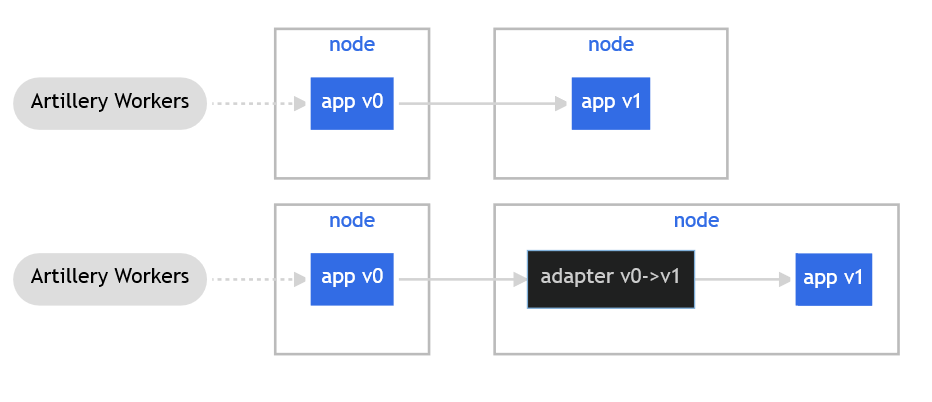
\includegraphics[height=2.4in]{pointExperiment}
    \caption{point-to-point experiment}
    \label{fig:gantt}
\end{figure}


\begin{figure}[htbp]
    \centering
    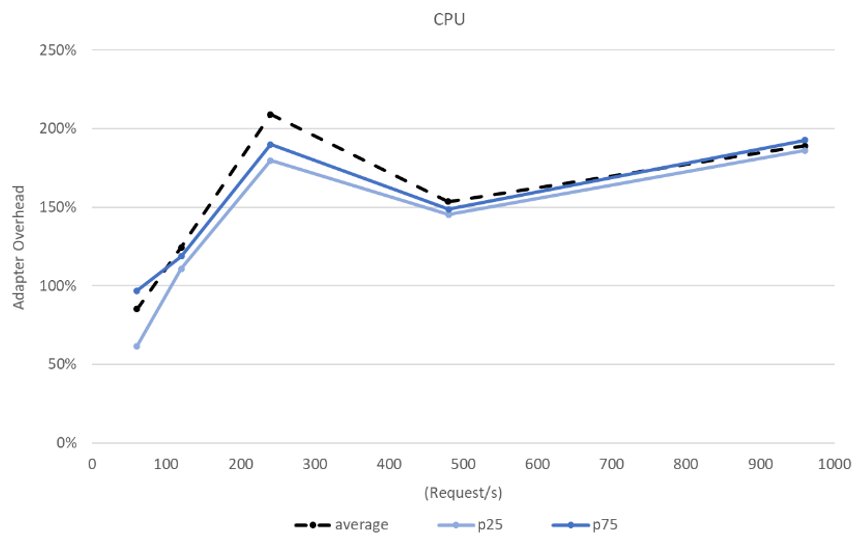
\includegraphics[height=3in]{Results/PtP/Cpu-PtP}
    \label{fig:gantt}
\end{figure}

\begin{figure}[htbp]
    \centering
    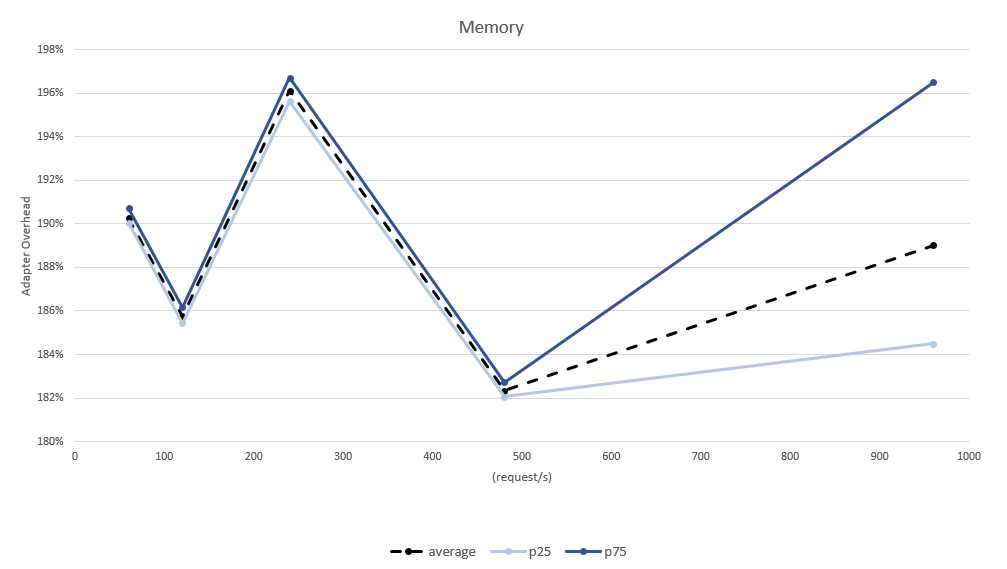
\includegraphics[height=3in]{Results/PtP/Memory-PtP}
    \label{fig:gantt}
\end{figure}

\begin{figure}[htbp]
    \centering
    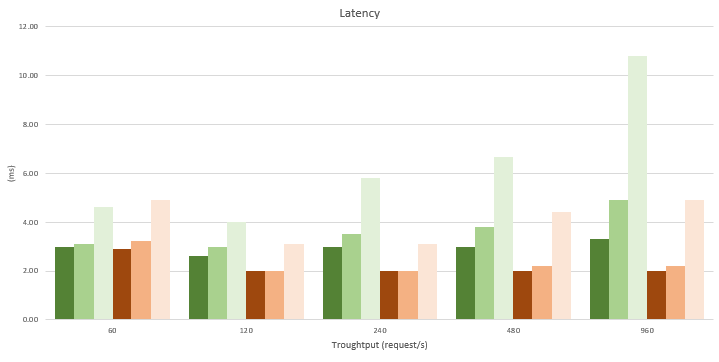
\includegraphics[height=3in]{Results/PtP/Latency-PtP}
    \label{fig:gantt}
\end{figure}

\begin{figure}[htbp]
    \centering
    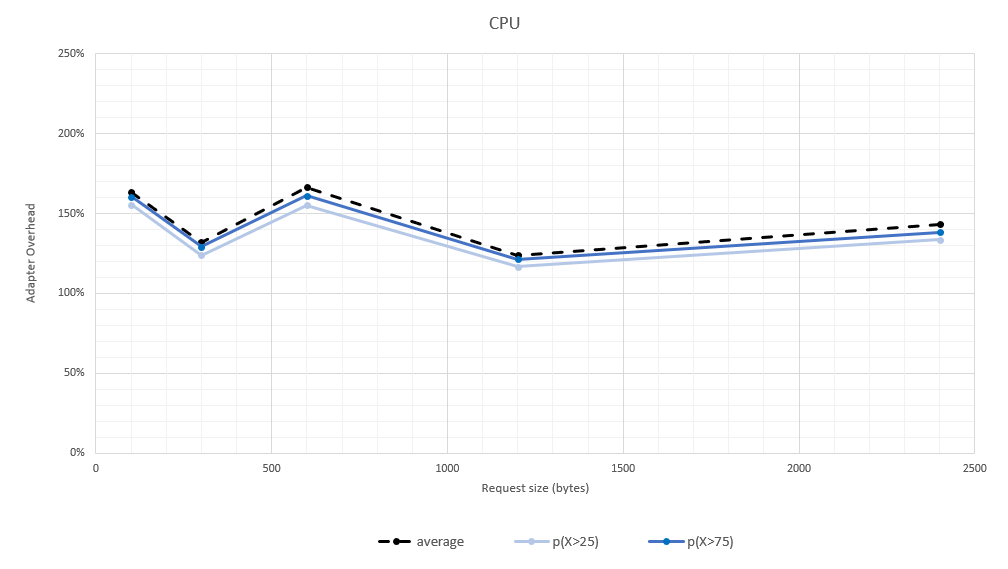
\includegraphics[height=3in]{Results/PtP_Size/Cpu-PtP_Size}
    \label{fig:gantt}
\end{figure}

\begin{figure}[htbp]
    \centering
    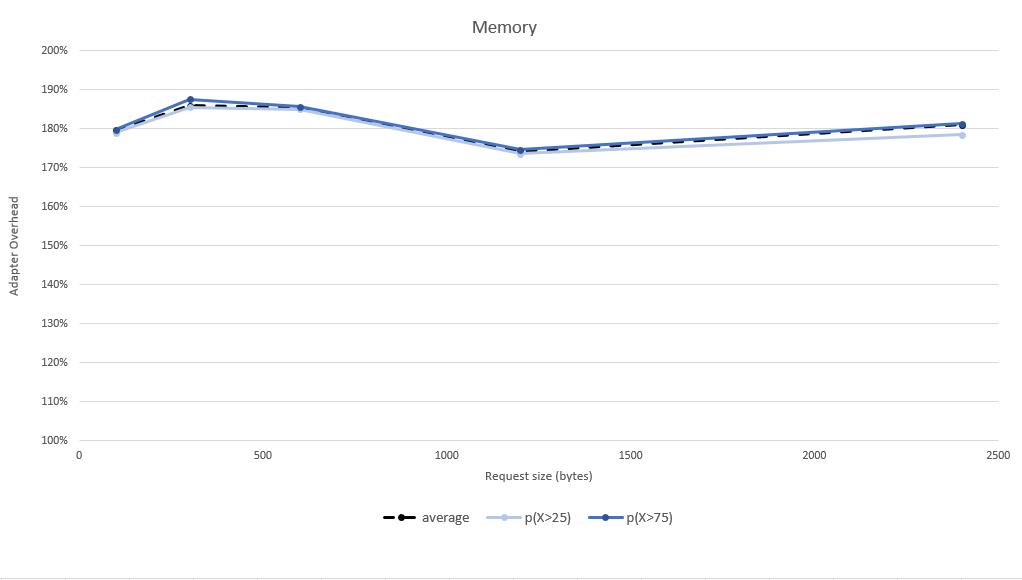
\includegraphics[height=3in]{Results/PtP_Size/Memory-PtP_Size}
    \label{fig:gantt}
\end{figure}

\begin{figure}[htbp]
    \centering
    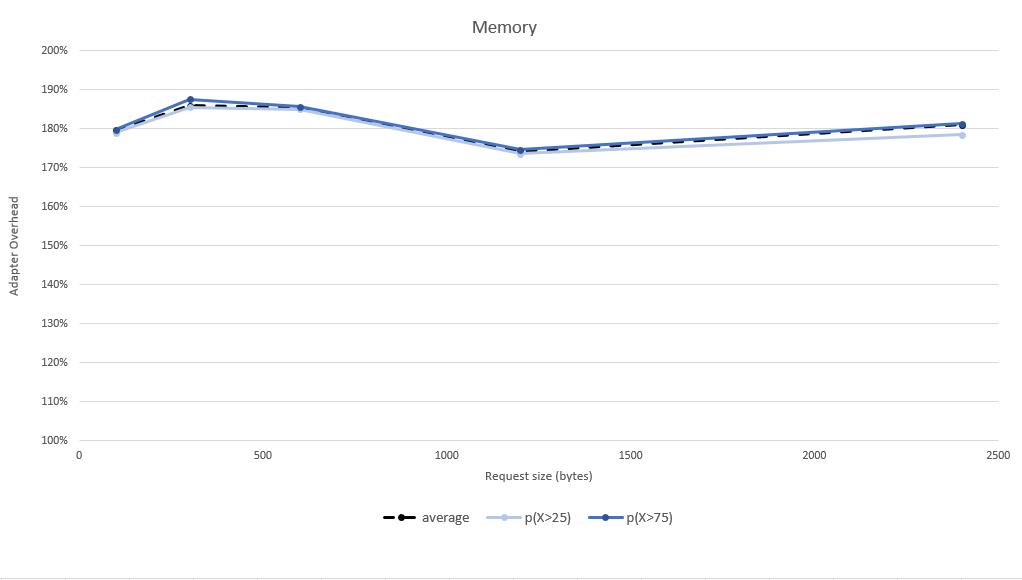
\includegraphics[height=3in]{Results/PtP_Size/Latency-PtP_Size}
    \label{fig:gantt}
\end{figure}

\begin{figure}[htbp]
    \centering
    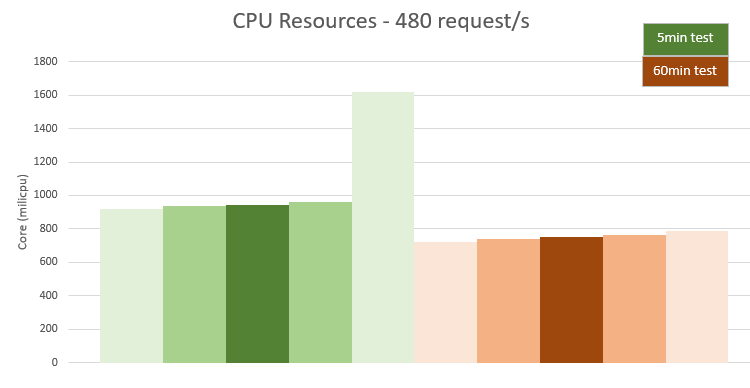
\includegraphics[height=3in]{Results/Ls/Cpu-Ls}
    \label{fig:gantt}
\end{figure}

\begin{figure}[htbp]
    \centering
    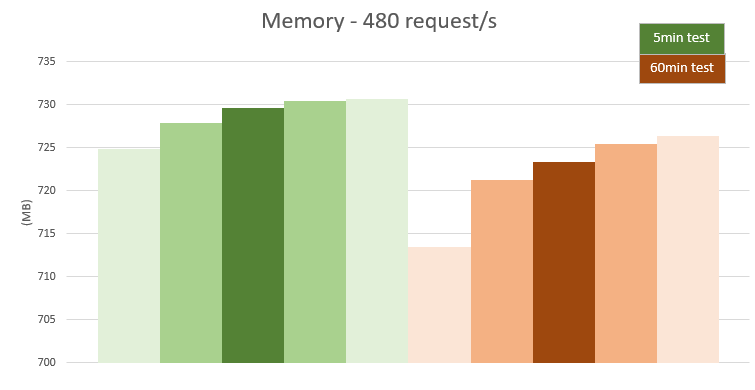
\includegraphics[height=3in]{Results/Ls/Memory-Ls}
    \label{fig:gantt}
\end{figure}

\begin{figure}[htbp]
    \centering
    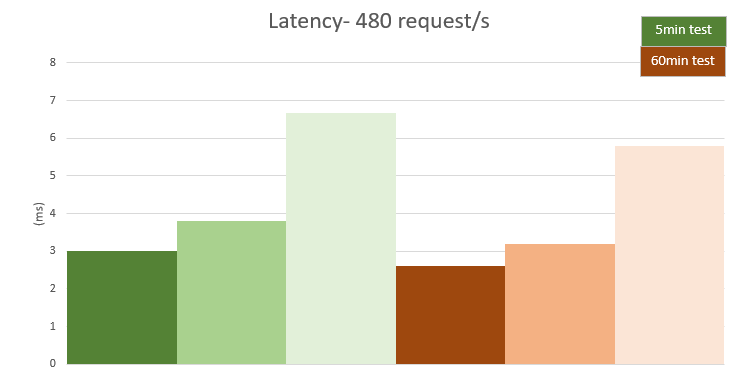
\includegraphics[height=3in]{Results/Ls/Latency-Ls}
    \label{fig:gantt}
\end{figure}

\newpage



\section{Weighted Point to Point} % (fold)
\label{sec:weighted point to point}

\begin{figure}[htbp]
    \centering
    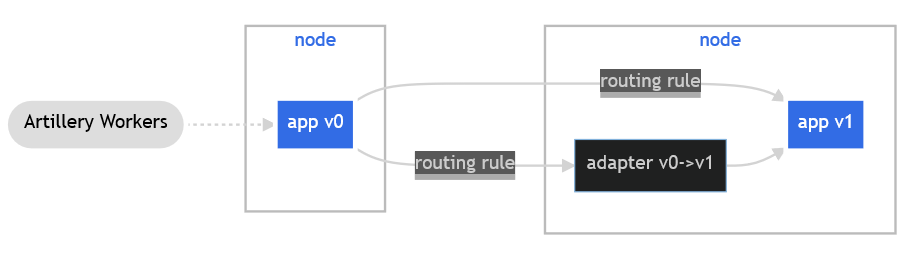
\includegraphics[height=1.8in]{routingExperiment}
    \caption{routing experiment}
    \label{fig:gantt}
\end{figure}

\begin{figure}[htbp]
    \centering
    \includegraphics[height=3in]{Results/R/Cpu-R}
    \label{fig:gantt}
\end{figure}

\begin{figure}[htbp]
    \centering
    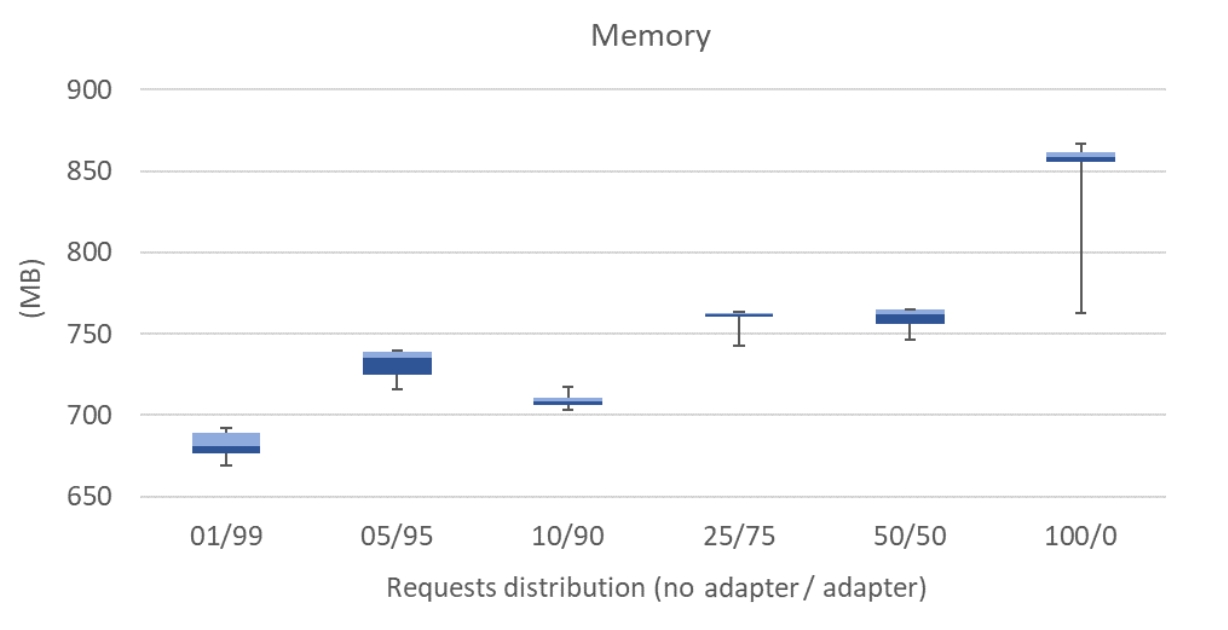
\includegraphics[height=3in]{Results/R/Memory-R}
    \label{fig:gantt}
\end{figure}

\begin{figure}[htbp]
    \centering
    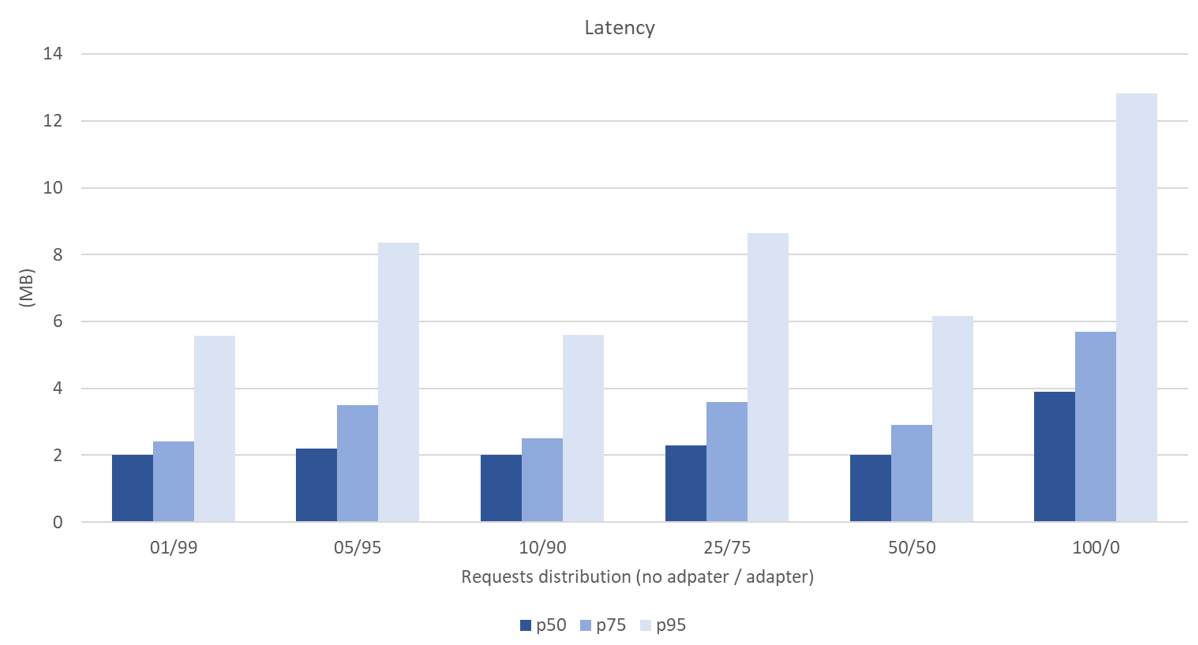
\includegraphics[height=3in]{Results/R/Latency-R}
    \label{fig:gantt}
\end{figure}

\newpage



\section{Bi-partition} % (fold)
\label{sec:bi-partition}

\begin{figure}[htbp]
    \centering
    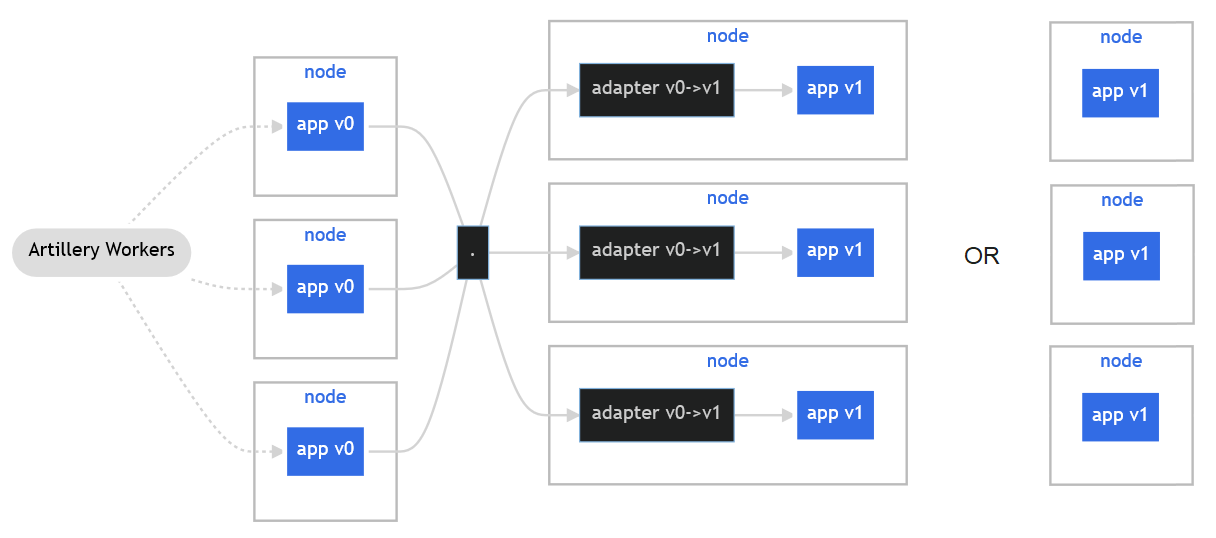
\includegraphics[height=2.7in]{bipartExperiment}
    \caption{bi-partition experiment}
    \label{fig:gantt}
\end{figure}

\begin{figure}[htbp]
    \centering
    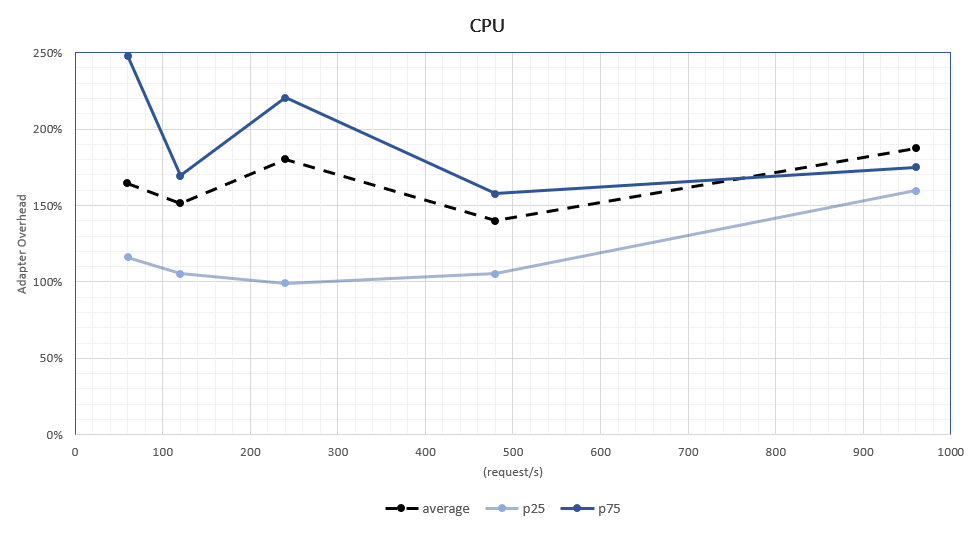
\includegraphics[height=4in]{Results/Bp/Cpu-Bp}
    \label{fig:gantt}
\end{figure}

\begin{figure}[htbp]
    \centering
    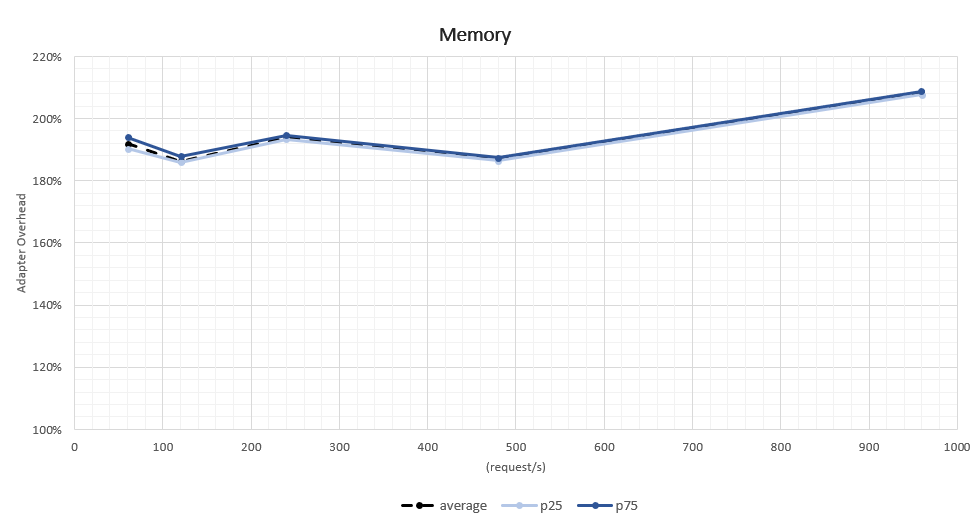
\includegraphics[height=4in]{Results/Bp/Memory-Bp}
    \label{fig:gantt}
\end{figure}

\begin{figure}[htbp]
    \centering
    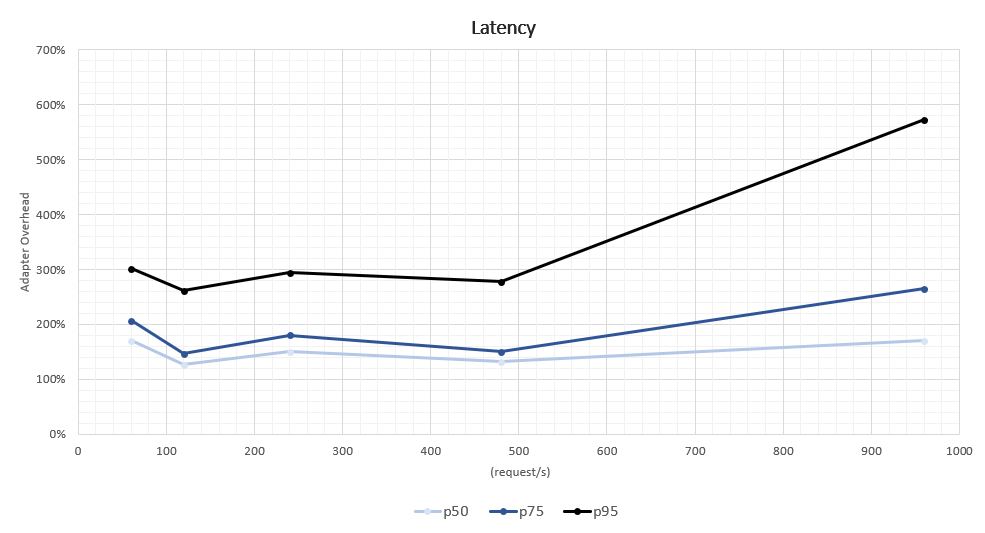
\includegraphics[height=3in]{Results/Bp/Latency-Bp}
    \label{fig:gantt}
\end{figure}

\section{Comparisons} % (fold)
\label{sec:comparisons}

\section{Conclusions} % (fold)
\label{sec:conclusions}